\documentclass[12pt]{report}
\usepackage[a4paper,margin=1in]{geometry}
\usepackage{graphicx}
\usepackage{fancyhdr}
\usepackage{titlesec}
\usepackage{amsmath, amssymb}
\usepackage{enumitem}
\usepackage{xcolor}
\usepackage{hyperref}
\usepackage{caption}
\usepackage{float}
\usepackage{listings}
\usepackage{tcolorbox}
\usepackage{booktabs}
\usepackage{longtable}
\usepackage[utf8]{inputenc}
\usepackage{array}
\usepackage{lipsum}
\usepackage{wrapfig}
\usepackage{tabularx}
\usepackage{tocloft}
\usepackage{setspace}
\usepackage{etoolbox}
\usepackage{sectsty}

% ---------------------------
% Odoo purple color
% ---------------------------
\definecolor{odooPurple}{RGB}{114,0,153}

% ---------------------------
% Header & footer
% ---------------------------
\fancypagestyle{plain}{
  \fancyhf{}
  \fancyfoot[C]{\thepage}
  \renewcommand{\headrulewidth}{0pt}
}

% ---------------------------
% Chapter / Section Styling
% ---------------------------
% Chapter title in purple with horizontal line
\titleformat{\chapter}[display]
  {\Huge\bfseries\color{odooPurple}}
  {\filleft\Huge\chaptertitlename~\thechapter}
  {1ex}
  {\filleft\color{odooPurple}}
  [\vspace{1ex}\color{odooPurple}\titlerule]

% Sections in actual chapters: purple bold
\titleformat{\section}{\Large\bfseries\color{odooPurple}}{\thesection}{1em}{}

% Subsections always black
\titleformat{\subsection}{\large\bfseries\color{black}}{\thesubsection}{1em}{}

% ---------------------------
% Body text in black
% ---------------------------
\color{black}

% ---------------------------
% Hyperref colors
% ---------------------------
\hypersetup{
    colorlinks=true,
    linkcolor=black, % TOC links color
    urlcolor=odooPurple,
    citecolor=odooPurple
}

% ---------------------------
% TOC styling
% ---------------------------
\setcounter{tocdepth}{2} % include sections

% Contents title: right-aligned, purple, horizontal line below
\renewcommand{\contentsname}{%
  \noindent\makebox[\textwidth][r]{\Huge\bfseries\color{odooPurple}Contents}%
}
\renewcommand{\cftaftertoctitle}{%
  \vspace{1em} % space below title
  \noindent\color{odooPurple}\rule{\textwidth}{1.5pt}\vspace{1em} % full-width line
}

% TOC entries
\renewcommand{\cftchapfont}{\bfseries\color{odooPurple}}      % chapters purple bold
\renewcommand{\cftchappagefont}{\bfseries\color{odooPurple}}  % chapter page numbers purple bold
\renewcommand{\cftsecfont}{\color{black}}                     % sections black normal
\renewcommand{\cftsecpagefont}{\color{black}}                 % section page numbers black normal
\renewcommand{\cftsecaftersnum}{.}                             % adds dot after section number

% Patch \tableofcontents to temporarily make sections black
\preto{\tableofcontents}{%
    \titleformat{\section}{\Large\bfseries\color{black}}{\thesection}{1em}{}%
}
\apptocmd{\tableofcontents}{%
    \titleformat{\section}{\Large\bfseries\color{odooPurple}}{\thesection}{1em}{}%
}{}{}

% ---------------------------
% Title page details
% ---------------------------
\title{
    \vspace*{2cm}
    \Huge\bfseries Coffee Chain ERP Manual\\[0.5cm]
    \LARGE\itshape Managing Outlets, Sales, CRM, and Menu Items with Odoo
}
\author{
    \large Author: Ravi Bhattarai\\[0.3cm]
    \large Co-Author: Nush Ojha
}
\date{\today}

% ---------------------------
% Part styling
% ---------------------------
\newcommand{\partpage}[1]{
    \clearpage
    \thispagestyle{empty}
    \vspace*{5cm}
    \begin{center}
        {\Huge\bfseries\color{odooPurple} #1\par}
    \end{center}
    \clearpage
}

% ---------------------------
% Document begins
% ---------------------------
\begin{document}

% ---------------------------
% Title page
% ---------------------------
\begin{titlepage}
    \centering
    \color{black} % All black on title page
    {\Huge\bfseries Coffee Chain ERP Manual\par}
    \vspace{1cm}
    {\LARGE\itshape Managing Outlets, Sales, CRM, and Menu Items with Odoo\par}
    \vspace{3cm}
    {\large Author: Ravi Bhattarai\par}
    \vspace{0.3cm}
    {\large Co-Author: Nush Ojha\par}
    \vfill
    {\large \today\par}
\end{titlepage}

% ---------------------------
% Preface
% ---------------------------
\chapter*{Preface}
\onehalfspacing
\color{black}
The Coffee Chain ERP is designed to streamline operations across multiple outlets while ensuring efficiency, transparency, and growth. This manual documents the structure, functionality, and guiding principles of the ERP system built on the Odoo platform. It is intended for developers, managers, and users responsible for operating and expanding the coffee chain.

The ERP integrates outlets, sales, CRM, and menu management into a single system. It provides performance metrics via sales reports, ensures role-based accountability, and allows modular expansion for future needs.

\newpage

% ---------------------------
% Table of Contents
% ---------------------------
\tableofcontents
\clearpage

% ---------------------------
% Part I: Strategic Foundation
% ---------------------------
\partpage{Part I: The Strategic Foundation}
\chapter{The TAO of the Odoo Coffee Chain Module: Guiding Philosophy}

More than just a software system, the Coffee Chain ERP embodies a philosophy that brings together people, processes, and purpose. Guided by the TAO, which emphasizes harmony and flow, the ERP aims to harmonize operational efficiency, customer delight, and organizational growth. In doing so, it ensures that every action within the coffee chain supports a broader vision of excellence, consistency, and sustainable progress.
\section{The Core Philosophy: Harmonizing People, Process, and Purpose}

The ERP’s philosophy is built on the understanding that technology should serve human intent, not dictate it. Its core principles include:

\begin{itemize}
    \item \textbf{Unified Vision:} All outlets, teams, and customer touchpoints are aligned within a single coherent framework. This creates a seamless experience for both staff and customers.  
    \item \textbf{Empowerment Through Clarity:} By providing clear visibility into operations, the ERP empowers managers and staff to act decisively and responsibly, transforming data into meaningful insights.  
    \item \textbf{Customer-Centric Mindset:} Every menu choice, transaction, and engagement is designed to enhance customer satisfaction, fostering loyalty and trust.  
    \item \textbf{Sustainable Growth:} Systems are conceived to support the coffee chain’s expansion, ensuring that scaling operations never compromises quality or culture.  
    \item \textbf{Harmony Between Technology and Human Judgment:} Automation is leveraged to reduce errors and inefficiencies, yet decisions remain guided by human insight and discretion.  
\end{itemize}

\section{Guiding Principles: The Values that Shape ERP Decisions}

These principles provide a moral and operational compass for the ERP, ensuring that daily actions align with strategic objectives:

\begin{itemize}
    \item \textbf{Simplicity and Elegance:} The system is designed to streamline complexity, presenting information and workflows in a clear, understandable manner.  
    \item \textbf{Transparency and Accountability:} Roles, responsibilities, and processes are explicit, enabling trust and fairness within teams.  
    \item \textbf{Continuous Improvement:} Insights and feedback from operations are used to refine processes, cultivating a culture of learning and excellence.  
    \item \textbf{Collaboration and Synergy:} Departments and outlets operate not as silos but as interconnected units, sharing knowledge and working toward common goals.  
    \item \textbf{Resilience and Adaptability:} The ERP encourages flexibility, allowing the organization to respond to changing market conditions, customer needs, or internal challenges without losing strategic focus.  
    \item \textbf{Integrity and Ethical Operations:} Every feature and process within the ERP is designed to maintain honesty, accuracy, and ethical treatment of data and customers.  
\end{itemize}

\section{Frame of Reference: Guiding the Coffee Chain Towards Excellence}

The ERP acts as a **philosophical and strategic lens** for decision-making, ensuring that operational choices reflect the chain’s broader mission:

\begin{itemize}
    \item \textbf{Strategic Alignment:} Every menu update, sales initiative, or customer engagement is anchored to long-term business objectives.  
    \item \textbf{Cultural Integration:} The ERP embodies the coffee chain’s values — quality, respect, and customer delight — reinforcing them in every interaction.  
    \item \textbf{Guided Flexibility:} While providing structure and consistency, the system allows local adaptation, enabling outlets to respond to unique customer demands while remaining aligned with the brand’s ethos.  
    \item \textbf{Forward-Looking Orientation:} Decisions made within the system are informed by foresight, preparing the organization for expansion, evolving customer preferences, and emerging market opportunities.  
    \item \textbf{Holistic Perspective:} Operations are viewed as part of a larger ecosystem, connecting outlets, teams, and customers in a continuous flow of value creation.  
\end{itemize}

\section*{Insights}

The philosophical foundation of the Coffee Chain ERP ensures that:  

\begin{itemize}
    \item Technology serves as a facilitator, harmonizing human judgment with operational processes.  
    \item Staff and managers are empowered with clarity, accountability, and purpose.  
    \item Customer experiences are consistently enhanced across all touchpoints.  
    \item Continuous improvement and learning are embedded into the organizational culture.  
    \item Growth and scalability are achieved without compromising operational excellence or brand integrity.  
    \item The ERP functions not just as a tool, but as a strategic partner in achieving the coffee chain’s vision.  
\end{itemize}
 % Chapter 1
\chapter{Strategic Context and Business Purpose}

This chapter provides a comprehensive view of the Coffee Chain ERP system, linking its strategic objectives with operational processes and highlighting the value it creates. It covers system context, process mapping, module roles, scope, and the problems addressed by the ERP, along with the tangible benefits it delivers to stakeholders.

\section{System Context (C4-Level 1): Departments, Roles, and Interactions}

Understanding the system context is the first step in appreciating how the ERP organizes and streamlines operations. The Coffee Chain ERP system aligns organizational departments into structured digital workflows, ensuring clarity in roles, accountability, and information flow across the entire coffee chain.

\subsection*{Departments Covered}
The ERP system organizes departmental responsibilities to ensure smooth coordination and operational efficiency (see Figure~\ref{fig:dept_interaction}):
\begin{itemize}
    \item \textbf{Outlet Management:} Maintains details of each coffee outlet such as name, location, and management assignments, ensuring visibility of operational capacity across the chain.
    \item \textbf{Sales:} Records daily transactions, revenue, and order details in real time to support operational monitoring and long-term planning.
    \item \textbf{Customer Relationship Management (CRM):} Tracks leads, customer details, and engagement history, enhancing marketing and customer retention.
    \item \textbf{Menu Management:} Provides a master list of products, categories, and pricing, synchronized with the sales process for consistent ordering.
\end{itemize}

\subsection*{Integration with QMS and PDCA}
The ERP embeds a quality-driven approach through the PDCA (Plan-Do-Check-Act) cycle. This ensures that departmental activities not only execute daily operations but also continuously improve processes:
\begin{itemize}
    \item \textbf{Plan:} Define objectives such as increasing sales, improving customer engagement, or optimizing outlet operations.
    \item \textbf{Do:} Execute daily activities through ERP modules, standardizing operations across all outlets.
    \item \textbf{Check:} Track performance indicators in dashboards to measure actual outcomes against planned objectives.
    \item \textbf{Act:} Managers adjust strategies, update menu items, or refine CRM tactics based on data-driven insights.
\end{itemize}

\begin{tcolorbox}[colback=white,colframe=odooPurple,title=Tip, fonttitle=\bfseries, coltitle=white]
Review KPIs weekly and use PDCA’s \textbf{Act} phase to refine outlet operations. 
Small, continuous improvements compound into significant performance gains.
\end{tcolorbox}

\subsection*{Interaction Diagram}
The interactions between departments are visually represented in Figure~\ref{fig:dept_interaction}, showing how the ERP facilitates seamless communication and data flow across all functional units.
\begin{figure}[H]
\centering
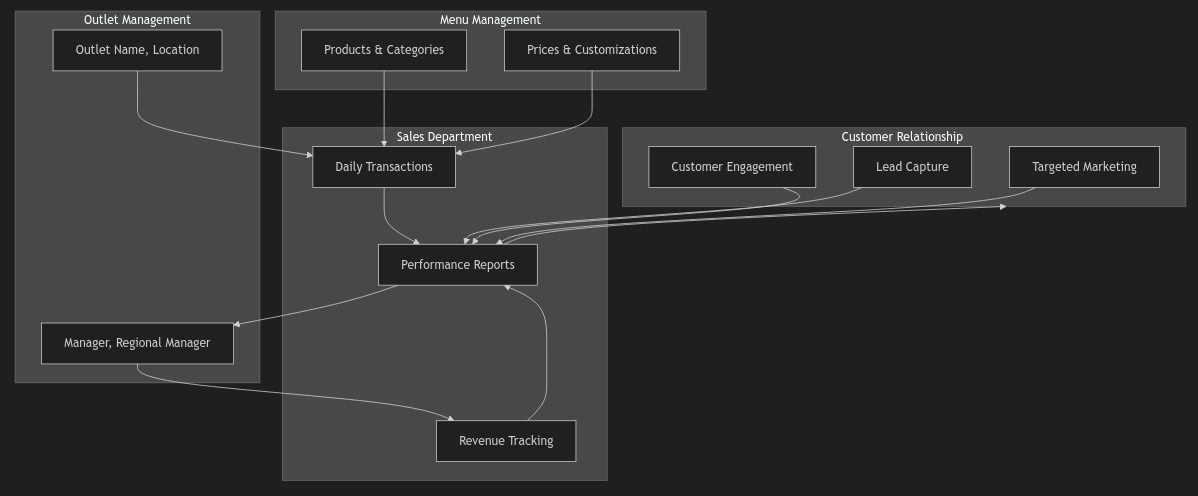
\includegraphics[width=0.9\textwidth,height=0.5\textheight,keepaspectratio]{diagrams/department.png}
\caption{Department Interaction Diagram of Coffee Chain ERP}
\label{fig:dept_interaction}
\end{figure}

\section{SIPOC Analysis: Mapping Processes and Stakeholders}

To further understand the ERP’s operational scope, the SIPOC framework provides a high-level process overview, highlighting Suppliers, Inputs, Processes, Outputs, and Customers (see Table~\ref{tab:sipoc_summary} and Figure~\ref{fig:sipoc_visual}). This ensures that all stakeholders and activities are mapped for clarity and efficiency.

\subsection*{Purpose of SIPOC}
The SIPOC analysis helps management visualize the end-to-end workflow and make informed decisions:
\begin{itemize}
    \item Identify key suppliers and inputs required for smooth operations.
    \item Understand critical processes that transform inputs into outputs.
    \item Ensure outputs meet customer expectations.
    \item Detect potential gaps or inefficiencies in the workflow.
\end{itemize}

\begin{tcolorbox}[colback=white,colframe=odooPurple,title=Tip, fonttitle=\bfseries, coltitle=white]
When conducting SIPOC analysis, involve representatives from all departments. 
This ensures that no critical input, process, or customer touchpoint is missed.
\end{tcolorbox}

\subsection*{Suppliers, Inputs, Processes, Outputs, Customers}

\subsubsection*{Suppliers}
\begin{itemize}
    \item \textbf{Coffee Outlets:} Provide sales data, menu updates, and operational feedback.
    \item \textbf{Suppliers:} Supply raw ingredients, coffee beans, and other consumables.
    \item \textbf{CRM:} Provides customer leads and engagement data for marketing and sales tracking.
\end{itemize}

\subsubsection*{Inputs}
\begin{itemize}
    \item Product details, pricing, and menu configurations.
    \item Raw materials and stock updates from suppliers.
    \item Customer leads and engagement information from the CRM.
\end{itemize}

\subsubsection*{Processes}
\begin{itemize}
    \item Tracking daily sales and updating the ERP system.
    \item Managing product and menu updates in real time.
    \item Receiving and logging stock from suppliers.
    \item Capturing customer interactions and monitoring CRM data.
\end{itemize}

\subsubsection*{Outputs}
\begin{itemize}
    \item Updated sales reports for each outlet and consolidated regional reports.
    \item Inventory reports and notifications for low-stock items.
    \item Real-time product updates for sales and POS systems.
    \item CRM insights for marketing and customer engagement.
\end{itemize}

\subsubsection*{Customers}
\begin{itemize}
    \item Management: Receives comprehensive reports for decision-making.
    \item Outlet Managers: Use outputs to manage day-to-day operations.
    \item Marketing/Sales Teams: Leverage CRM insights to plan campaigns.
    \item Customers: Benefit indirectly through accurate pricing, better product availability, and consistent service.
\end{itemize}

\subsection*{SIPOC Table}
The structured SIPOC table below summarizes the relationships between suppliers, inputs, processes, outputs, and customers:
\begin{table}[H]
\centering
\begin{tabular}{|p{3cm}|p{3cm}|p{4cm}|p{3cm}|p{3cm}|}
\hline
\textbf{Suppliers} & \textbf{Inputs} & \textbf{Process} & \textbf{Outputs} & \textbf{Customers} \\
\hline
Coffee outlets & Product & Track sales, update ERP, manage orders & Sales reports, product updates & Management, Customers \\
\hline
Suppliers & Ingredients, stock & Receive and log stock in ERP & Updated inventory & Outlet managers, Kitchen staff \\
\hline
CRM & Customer leads & Capture and manage leads & Lead reports, CRM data & Marketing, Sales team \\
\hline
\end{tabular}
\caption{SIPOC for Coffee Chain ERP}
\label{tab:sipoc_summary}
\end{table}

\subsection*{Visual SIPOC Diagram}
The visual representation in Figure~\ref{fig:sipoc_visual} provides an intuitive understanding of process flow and interdependencies.
\begin{figure}[H]
\centering
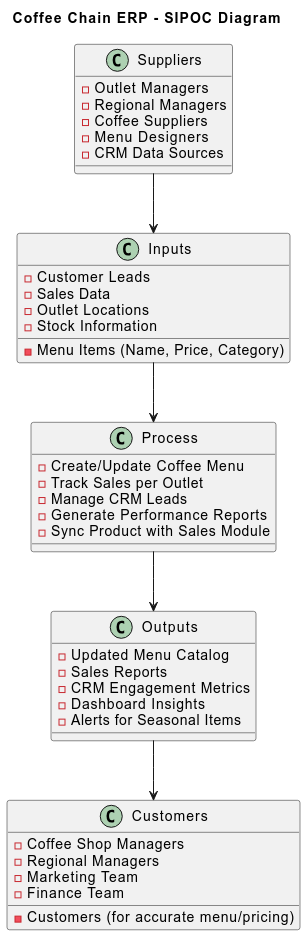
\includegraphics[width=0.85\textwidth,height=0.6\textheight,keepaspectratio]{diagrams/SIPOC.png}
\caption{Visual SIPOC Diagram of Coffee Chain ERP}
\label{fig:sipoc_visual}
\end{figure}

\section{Module Role and Scope: Defining Responsibilities and Boundaries}

Having established the system context and process flows, it is essential to define the module’s role and scope to clarify responsibilities and set boundaries for operational functionality.

\subsection*{Role of the ERP Module}
The Coffee Chain ERP acts as an integrative backbone for all coffee chain operations:
\begin{itemize}
    \item \textbf{Unification:} Combines outlet, menu, sales, and CRM functions into one system.  
    \item \textbf{Consistency:} Ensures standardized processes across all outlets.  
    \item \textbf{Insight:} Provides managers with real-time and historical data for decision-making.  
    \item \textbf{Scalability:} Prepares the system for future growth, such as adding loyalty features or advanced analytics.  
\end{itemize}

\subsection*{Scope of the Coffee Chain ERP}
\begin{itemize}
    \item Covers active coffee outlets and their daily operations.  
    \item Includes menu item management, pricing, and categorization.  
    \item Captures all sales orders and integrates them with reporting dashboards.  
    \item Synchronizes CRM data with sales transactions for lead tracking.  
    \item Excludes loyalty and reward systems, outlet capacity tracking, and HR functions.  
\end{itemize}

\begin{tcolorbox}[colback=white,colframe=odooPurple,title=Tip, fonttitle=\bfseries, coltitle=white]
Clearly communicate module scope to all stakeholders. 
This avoids scope creep, prevents misaligned expectations, and ensures efficient ERP implementation.
\end{tcolorbox}

\subsection*{Stakeholders and KPIs}
\begin{itemize}
    \item \textbf{Outlet Managers:} Track efficiency and revenue.  
          \textit{KPIs: daily revenue, sales per product.}
    \item \textbf{Regional Managers:} Compare multiple outlets.  
          \textit{KPIs: average outlet growth, variance analysis.}
    \item \textbf{Employees:} Maintain data quality.  
          \textit{KPIs: error rate in transactions, product data accuracy.}
    \item \textbf{Top Management:} Align operations with strategy.  
          \textit{KPIs: conversion rates, long-term revenue growth.}
\end{itemize}

\subsection*{Context Diagram (C1)}
The C1-level context diagram (Figure~\ref{fig:c1_context}) illustrates the module boundaries and interactions between stakeholders and system components.
\begin{figure}[H]
\centering
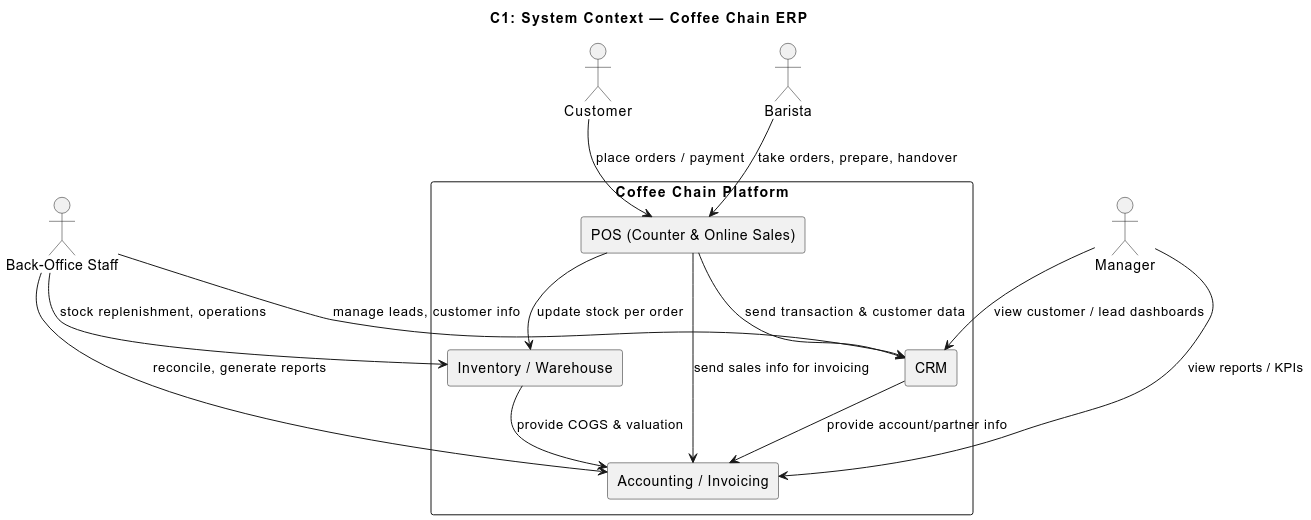
\includegraphics[width=0.9\textwidth,keepaspectratio]{diagrams/context.png}
\caption{C1-Level Context Diagram of Coffee Chain ERP}
\label{fig:c1_context}
\end{figure}

\section{The Pain-Gain Canvas: Problems Solved and Value Created by the Module}

Finally, the Pain-Gain Canvas provides a structured overview of operational challenges (Pains) and the tangible value (Gains) delivered by the ERP system, connecting directly to the system’s role and scope.

\subsection*{Pains: Operational Challenges}
\begin{itemize}
    \item Manual sales tracking across outlets.
    \item Menu updates not automatically reflected in sales.
    \item Limited visibility into customer leads and engagement.
    \item Difficulty generating consolidated reports.
    \item Data entry and pricing errors.
    \item Fragmented CRM data across outlets.
\end{itemize}

\subsection*{Gains: Value Additions}
\begin{itemize}
    \item Centralized ERP platform integrating outlets, sales, menu, and CRM.
    \item Real-time menu updates across all sales channels.
    \item Automated reporting dashboards with actionable metrics.
    \item Enhanced decision-making via consolidated and accurate information.
    \item Improved customer engagement through centralized CRM.
    \item Reduced errors via automation of pricing, stock management, and sales tracking.
\end{itemize}

\begin{tcolorbox}[colback=white,colframe=odooPurple,title=Tip, fonttitle=\bfseries, coltitle=white]
Revisit the Pain-Gain Canvas quarterly. 
Business needs evolve, and aligning ERP functionality with changing pains ensures continued ROI.
\end{tcolorbox}

\subsection*{Visual Pain-Gain Canvas}
The visual Pain-Gain Canvas (Figure~\ref{fig:pain_gain}) reinforces the connection between operational challenges and system benefits.
\begin{figure}[H]
\centering
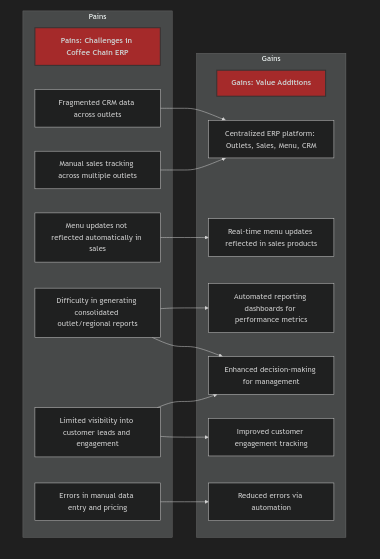
\includegraphics[width=0.85\textwidth,height=0.6\textheight,keepaspectratio]{diagrams/pain_gain.png}
\caption{Pain-Gain Canvas of Coffee Chain ERP}
\label{fig:pain_gain}
\end{figure}

\section*{Insights}

Bringing together system context, process mapping, role and scope, and the Pain-Gain Canvas, the Coffee Chain ERP demonstrates clear strategic value:

\begin{itemize}
    \item Departments are digitally connected, reducing data fragmentation and ensuring clarity in responsibilities.
    \item ERP modules unify operations, enforce consistency, and provide scalability for future growth.
    \item SIPOC analysis highlights key process dependencies, integration points, and potential operational bottlenecks.
    \item Pain-Gain analysis demonstrates how the ERP resolves operational challenges while delivering tangible benefits for management, staff, and customers.
    \item KPIs and dashboards provide actionable insights to support data-driven decision-making.
    \item Integration with QMS and PDCA ensures continuous improvement across all outlets.
    \item Overall, the ERP ensures smooth daily operations, real-time visibility into sales, menu, and CRM data, improved customer engagement, and strategic alignment across the coffee chain.
\end{itemize}
 % Chapter 2

% ---------------------------
% Part II: Architectural and Conceptual Framework
% ---------------------------
\partpage{Part II: Architectural and Conceptual Framework}
\chapter{Components \& Containers}

This chapter provides a detailed breakdown of the Coffee Chain ERP system in terms of its \textbf{containers} (modules) and the internal \textbf{components} of each module. Understanding the containers and components is essential for grasping the system architecture and how different parts interact to achieve operational efficiency.

\section*{Definition of a Container}

In the context of Coffee Chain ERP, a \textbf{container} represents a deployable or executable part of the system, such as a web application, microservice, or database, that encapsulates a set of functionality. Containers can be thought of as the high-level building blocks of the system. For example, the Sales Module is a container because it is a standalone web application managing sales transactions, linked to menu and CRM modules.

\section*{Containers of Coffee Chain ERP (C2 Diagram)}

The following containers constitute the Coffee Chain ERP system:

\begin{itemize}
    \item \textbf{Outlet Management:} Web application managing outlet details, managers, and regional assignments.
    \item \textbf{Sales Module:} Web application capturing daily sales, linking products to orders, and generating performance reports.
    \item \textbf{CRM Module:} Web application tracking customer leads, interactions, and supporting targeted marketing.
    \item \textbf{Menu Module:} Web application managing products, categories, and prices, synchronized with Sales.
    \item \textbf{Reporting \& Analytics:} Web application providing dashboards and consolidated performance insights.
\end{itemize}

\begin{figure}[H]
\centering
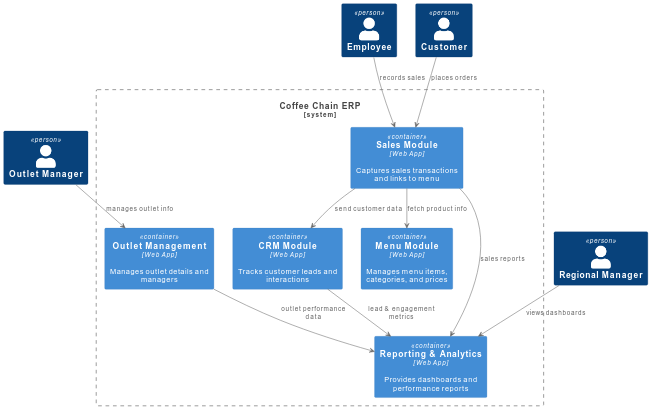
\includegraphics[width=0.9\textwidth,keepaspectratio]{diagrams/C2.png}
\caption{C2-Level Container Diagram of Coffee Chain ERP}
\end{figure}

\subsection*{Insights}

The C2 diagram illustrates how each module (container) interacts with other modules and external actors (employees, managers, customers). This high-level view helps stakeholders understand dependencies, system boundaries, and data flow without needing to inspect individual module internals.

\section*{Components of Each Container (C3 Diagrams)}

Each container is composed of internal components that define its functionality and interactions. These components are depicted in C3-level component diagrams.

\subsection*{Outlet Management Module Components}
\begin{itemize}
    \item Outlet Information Management
    \item Manager Assignment Component
    \item Regional Performance Component
    \item Reporting Component
\end{itemize}

\begin{figure}[H]
\centering
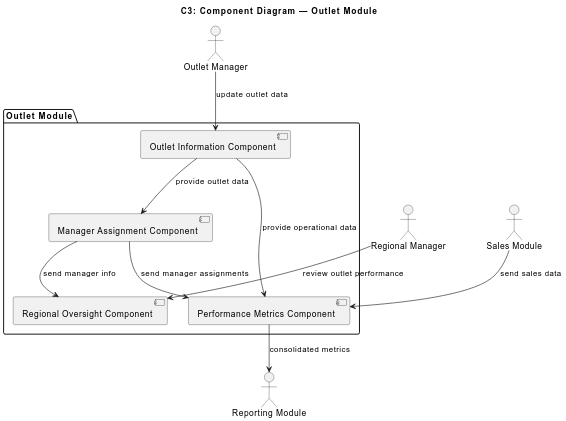
\includegraphics[width=0.9\textwidth,keepaspectratio]{diagrams/C3_outlet.png}
\caption{C3-Level Component Diagram — Outlet Management}
\end{figure}

\subsection*{Sales Module Components}
\begin{itemize}
    \item Transaction Processing Component
    \item Reporting Component
    \item Product Link Component
    \item Payment Processing Component
\end{itemize}

\begin{figure}[H]
\centering
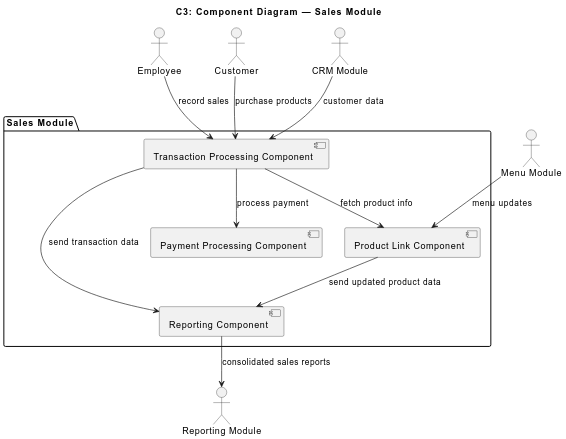
\includegraphics[width=0.9\textwidth,keepaspectratio]{diagrams/C3_sales.png}
\caption{C3-Level Component Diagram — Sales Module}
\end{figure}

\subsection*{CRM Module Components}
\begin{itemize}
    \item Lead Management Component
    \item Customer Interaction Component
    \item Customer Segmentation Component
    \item CRM Reporting Component
\end{itemize}

\begin{figure}[H]
\centering
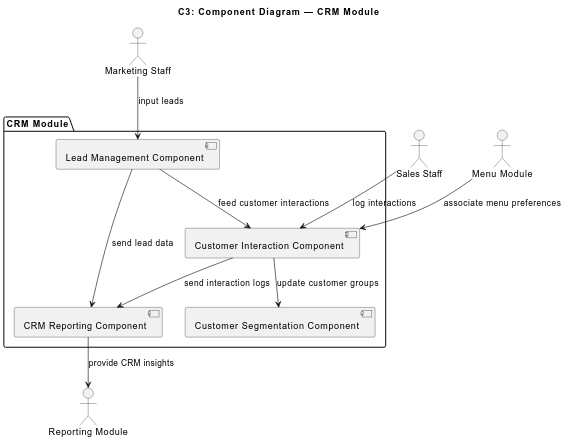
\includegraphics[width=0.9\textwidth,keepaspectratio]{diagrams/C3_crm.png}
\caption{C3-Level Component Diagram — CRM Module}
\end{figure}

\subsection*{Menu Module Components}
\begin{itemize}
    \item Menu Item Management Component
    \item Category Management Component
    \item Pricing Component
    \item Menu-Sales Synchronization Component
\end{itemize}

\begin{figure}[H]
\centering
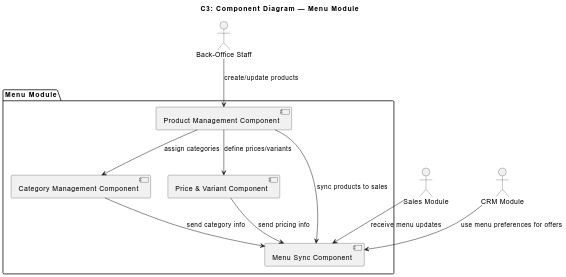
\includegraphics[width=0.9\textwidth,keepaspectratio]{diagrams/C3_menu.png}
\caption{C3-Level Component Diagram — Menu Module}
\end{figure}

\subsection*{Insights}

Analyzing the C3 diagrams reveals the following:

\begin{itemize}
    \item Each module has a clear separation of responsibilities via components.
    \item Internal components communicate with external actors (employees, customers, managers) and other modules to provide seamless operations.
    \item The ERP system’s modular architecture enables future extension, such as adding Loyalty \& Rewards or Inventory Management, without disrupting existing modules.
    \item Real-time synchronization between Menu, Sales, and CRM is critical for accurate reporting and decision-making.
\end{itemize}

   % Chapter 3
\chapter{Components \& Integration}  % Chapter 4
\chapter{Concepts \& Documentation}

This chapter introduces the key concepts behind the Coffee Chain ERP system and details the important documents and records used in the workflow. Understanding these concepts is essential for grasping how the ERP operates and how data flows between modules.

\section*{Key Concepts}

\subsection*{1. ERP System Integration}
The Coffee Chain ERP is designed as an integrated platform combining multiple business functions—outlet management, sales, menu management, and CRM. Integration ensures that updates in one module automatically propagate to others, reducing manual work and errors.  

\textbf{Example:} Updating a menu item in the Menu module automatically updates the Sales module, ensuring that employees sell the correct items with accurate pricing.

\subsection*{2. Module-Based Architecture}
The ERP is organized into distinct modules (containers) and components:

\begin{itemize}
    \item \textbf{Outlet Management:} Stores information about each coffee outlet, including name, location, manager, and regional manager.
    \item \textbf{Sales Module:} Handles transactions, product linking, and performance reporting.
    \item \textbf{Menu Module:} Manages products, categories, and pricing, linking to the Sales module.
    \item \textbf{CRM Module:} Tracks customer leads, interactions, and engagement metrics.
    \item \textbf{Reporting \& Analytics:} Consolidates data from all modules for dashboards and decision support.
\end{itemize}

\subsection*{3. Workflow Concepts}
\begin{itemize}
    \item \textbf{Transaction Flow:} From order placement to sales recording, each step is logged in the ERP for accuracy.
    \item \textbf{Data Synchronization:} Changes in one module (e.g., menu updates) reflect immediately in dependent modules (e.g., sales).
    \item \textbf{Decision Support:} Consolidated reports allow managers and regional managers to track KPIs such as revenue, product sales, and lead conversion rates.
\end{itemize}

\subsection*{4. User Roles and Responsibilities}
\begin{itemize}
    \item \textbf{Outlet Managers:} Manage outlet operations and ensure accurate data entry.
    \item \textbf{Regional Managers:} Compare performance across outlets and make strategic decisions.
    \item \textbf{Employees:} Enter sales and product information accurately.
    \item \textbf{Customers:} Interact with the system via orders; indirectly feed CRM data.
\end{itemize}

\subsection*{5. Concept of Containers and Components}
In this ERP context:
\begin{itemize}
    \item A \textbf{Container} represents a high-level module such as Sales, CRM, or Menu.
    \item A \textbf{Component} is a sub-part of a container that executes a specific function, e.g., the \emph{Transaction Processing Component} in Sales.
\end{itemize}

\section*{Documents in the Workflow}

\subsection*{1. Sales Records}
\begin{itemize}
    \item Captured automatically by the Sales module.
    \item Includes transaction ID, product sold, quantity, price, payment method, and timestamp.
    \item Serves as the basis for financial reports and performance analytics.
\end{itemize}

\subsection*{2. Menu Master List}
\begin{itemize}
    \item Contains all products, categories, and pricing information.
    \item Maintained in the Menu module; synchronized with Sales.
    \item Provides consistency in product offerings across outlets.
\end{itemize}

\subsection*{3. Customer \& Lead Records}
\begin{itemize}
    \item Captured by the CRM module.
    \item Includes lead source, customer information, interaction logs, and engagement metrics.
    \item Used for marketing, promotions, and improving customer relationships.
\end{itemize}

\subsection*{4. Outlet Data Sheets}
\begin{itemize}
    \item Contains outlet details: name, location, manager, regional manager.
    \item Maintained in the Outlet Management module.
    \item Supports reporting and operational oversight.
\end{itemize}

\subsection*{5. Reports and Dashboards}
\begin{itemize}
    \item Generated by the Reporting \& Analytics module.
    \item Summarizes sales, outlet performance, and customer engagement.
    \item Provides actionable insights for decision-making.
\end{itemize}

\section*{Integration of Documents with Modules}

\begin{itemize}
    \item Sales records are linked to menu items and CRM leads.
    \item Customer engagement documents feed into reporting dashboards.
    \item Outlet data is referenced for KPI calculation and performance benchmarking.
\end{itemize}

\section*{Code and Diagram Integration}

\begin{lstlisting}[language=Python, caption={Example: Sales Transaction Recording in Python}]
class SaleOrder(models.Model):
    _inherit = 'sale.order'

    outlet_id = fields.Many2one('coffee.outlet', string='Outlet')
    customer_id = fields.Many2one('res.partner', string='Customer')
\end{lstlisting}

\begin{figure}[H]
\centering
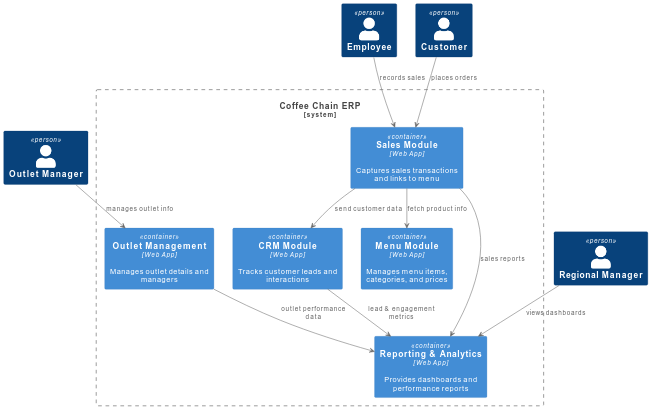
\includegraphics[width=0.9\textwidth,keepaspectratio]{diagrams/C2.png}
\caption{Reference Container Diagram for Document Flow}
\end{figure}

\section*{Insights}

\begin{itemize}
    \item Centralizing document management reduces errors and ensures data consistency.
    \item Clear linkage between documents and modules enhances traceability and decision-making.
    \item Automated capture of sales, menu, and customer data minimizes manual intervention.
    \item Reporting dashboards serve as the single source of truth for management insights.
\end{itemize}
      % Chapter 5
\chapter{Workflow and Customer Journey for Coffee Chain ERP System}

\section*{Introduction}
This chapter describes the workflow and customer journey in the Coffee Chain ERP system. The system is designed to manage coffee outlets, menu items, sales orders, and customer information. The goal is to provide a clear understanding of how users (staff and administrators) interact with the system and how sale customers experience the ordering process.

\section*{System Entities}
The main entities in the Coffee Chain ERP system are:

\begin{itemize}
    \item \textbf{Coffee Outlet (\texttt{coffee.outlet})}: Represents a coffee outlet in the chain.
    \item \textbf{Outlet Owner (\texttt{res.partner})}: Represents the owner of a coffee outlet.
    \item \textbf{Coffee Menu Item (\texttt{coffee.menu.item})}: Represents drinks and snacks available for order.
    \item \textbf{Sale Customer (\texttt{res.partner})}: Represents the end customer purchasing products at the outlet.
    \item \textbf{Sale Order (\texttt{sale.order})}: Represents a customer's order in the system.
    \item \textbf{CRM Lead (\texttt{crm.lead})}: Optional linkage for sales leads and customer management.
\end{itemize}

\section*{Workflow Sequence}
The workflow represents the operations performed by administrators and staff for managing outlets, menu items, customers, and sales orders.

\subsection*{Administrator Workflow}
Administrators are responsible for setting up outlets, outlet owners, and menu items. The workflow is as follows:

\begin{enumerate}
    \item Create or manage \textbf{Outlet Owner} (\texttt{res.partner}).
    \item Create or view a \textbf{Coffee Outlet} and assign it to an outlet owner.
    \item Create \textbf{Menu Items} (drinks and snacks) that can later be added to customer orders.
    \item Create or manage \textbf{Sale Customers} (\texttt{res.partner}) who purchase items at the outlet.
    \item Optionally link \textbf{CRM Leads} to track customer interactions.
\end{enumerate}

\begin{figure}[H]
    \centering
    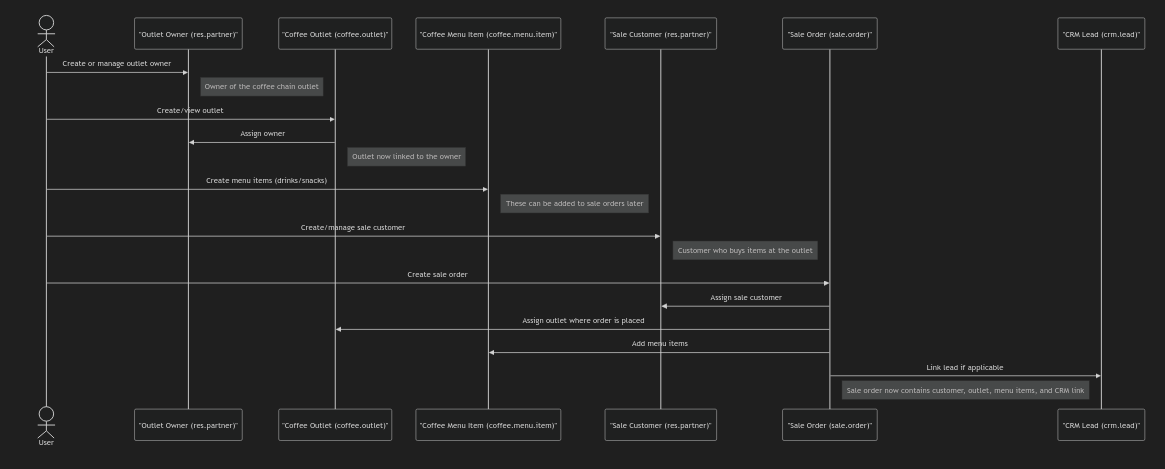
\includegraphics[width=0.85\textwidth]{diagrams/sequence.png}
    \caption{Administrator Workflow Sequence Diagram}
\end{figure}

\section*{Customer Journey}
The customer journey demonstrates how a sale customer interacts with the coffee outlet via the staff (barista) using the POS system.

\subsection*{Steps in the Customer Journey}
\begin{enumerate}
    \item Customer approaches the outlet and places an order with the staff.
    \item Staff identifies the outlet where the order is being placed.
    \item Staff adds the selected menu items to a \textbf{Sale Order}.
    \item Sale order is linked to the outlet and optionally to a CRM lead.
    \item Customer makes payment to the staff.
    \item Staff confirms the order and issues a receipt.
    \item Sale is recorded in the system, including customer details, menu items, outlet, and CRM link if applicable.
\end{enumerate}

\begin{figure}[H]
    \centering
    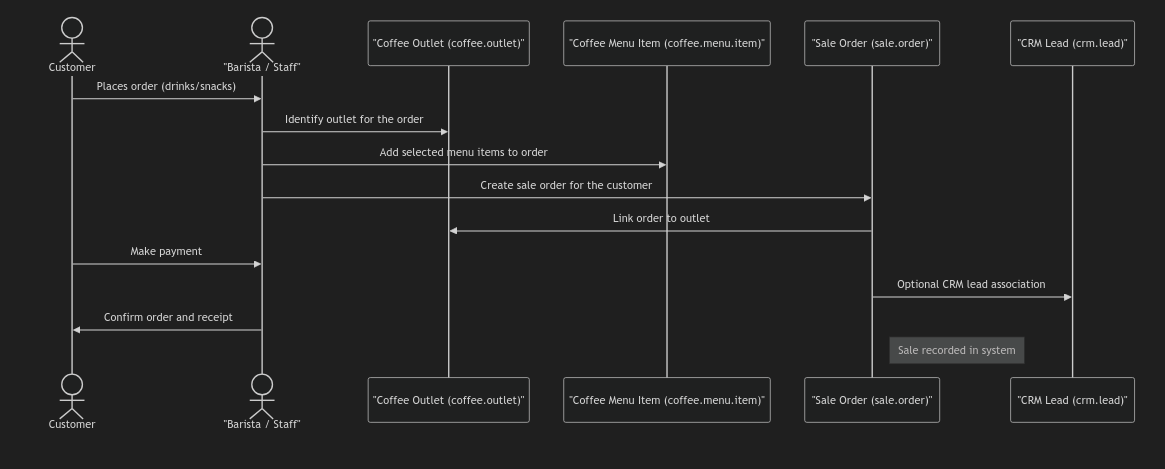
\includegraphics[width=0.85\textwidth]{diagrams/customer_journey.png}
    \caption{Customer Journey Sequence Diagram}
\end{figure}


This chapter provided a detailed workflow and customer journey for the Coffee Chain ERP system. By separating the \textbf{administrator workflow} from the \textbf{customer journey}, the system clearly defines responsibilities and interactions:

\begin{itemize}
    \item Administrators manage outlets, owners, and menu items.
    \item Staff (baristas) enter orders and process payments on behalf of customers.
    \item Sale orders record all interactions with outlets, menu items, customers, and optionally CRM leads.
\end{itemize}

                % Chapter 6
\chapter{Configuration \& Business Logic}

\section*{Module Configuration}

\subsection*{Coffee Outlet}
Each coffee outlet has a digital record in the ERP. Key configurations include:
\begin{itemize}
    \item \textbf{Outlet Name:} The unique identifier of the branch.
    \item \textbf{Location:} Physical address used for reporting and mapping.
    \item \textbf{Manager:} Linked to an employee in the system.
    \item \textbf{Integration with Sales:} Outlets are associated with each sales order for proper reporting and revenue tracking.
\end{itemize}

\subsection*{Coffee Menu Items}
The menu module defines all items sold in outlets. Configuration fields include:
\begin{itemize}
    \item \textbf{Name:} The item name (required).
    \item \textbf{Price:} Set in the company currency; used in sales orders.
    \item \textbf{Category:} Drinks, Snacks, Desserts, or Vegan.
    \item \textbf{Status:} Draft, Active, Seasonal, or Retired.
    \item \textbf{Image:} Optional image for kanban or POS display.
    \item \textbf{Customization Options:} Milk type, size, syrup flavor, and extra shot.
    \item \textbf{Linked Product:} Each menu item automatically creates/updates a `product.product` record for integration with the sales and accounting modules.
\end{itemize}

\subsection*{Access Control}
\begin{itemize}
    \item Users with the \texttt{access\_coffee\_menu\_item\_user} or \texttt{access\_coffee\_menu\_tag\_user} groups can create, read, write, and delete menu items or tags.
    \item Manager-level permissions can be configured in Odoo's security groups for outlets and sales.
\end{itemize}



\section*{Business Logic}

\subsection*{Menu Item Lifecycle}
\begin{itemize}
    \item When a menu item is created, the system automatically generates a linked product in the Odoo product catalog.
    \item Updates to price, name, or category propagate to the linked product.
    \item Deleting or retiring a menu item ensures it is no longer selectable in sales transactions.
\end{itemize}

\subsection*{Sales Order Integration}
\begin{itemize}
    \item Each sales order references the outlet (`coffee.outlet`) and customer (`res.partner`) directly.
    \item Items added to the order are linked to the `product.product` created by the menu module.
    \item This ensures correct pricing and consistency between menu configuration and sales transactions.
\end{itemize}

\subsection*{Customization Handling}
\begin{itemize}
    \item Customer preferences (milk type, size, syrup flavor, extra shot) are stored per order line.
    \item These preferences do not create new products but are saved in order notes for outlet preparation.
\end{itemize}

\subsection*{Tagging Logic}
\begin{itemize}
    \item Menu items can be assigned tags (`coffee.menu.tag`) for categorization or filtering in POS and reports.
    \item Tags are independent and reusable across multiple items.
\end{itemize}

\section*{Recommended Diagrams}
\begin{itemize}
    \item \textbf{Flow Diagram:} Shows the creation of a menu item and automatic product linkage.
    \item \textbf{Sequence Diagram:} Illustrates a sales order being placed, linking outlet, customer, and menu item.
\end{itemize}

\begin{figure}[H]
\centering
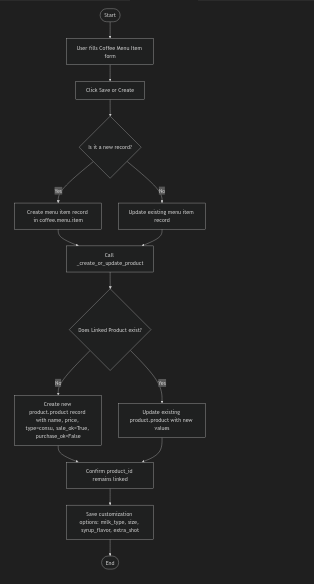
\includegraphics[width=0.6\textwidth,keepaspectratio]{diagrams/flowdiagram.png}
\caption{Flow Diagram: Menu Item Creation and Product Linkage}
\end{figure}

\begin{figure}[H]
\centering
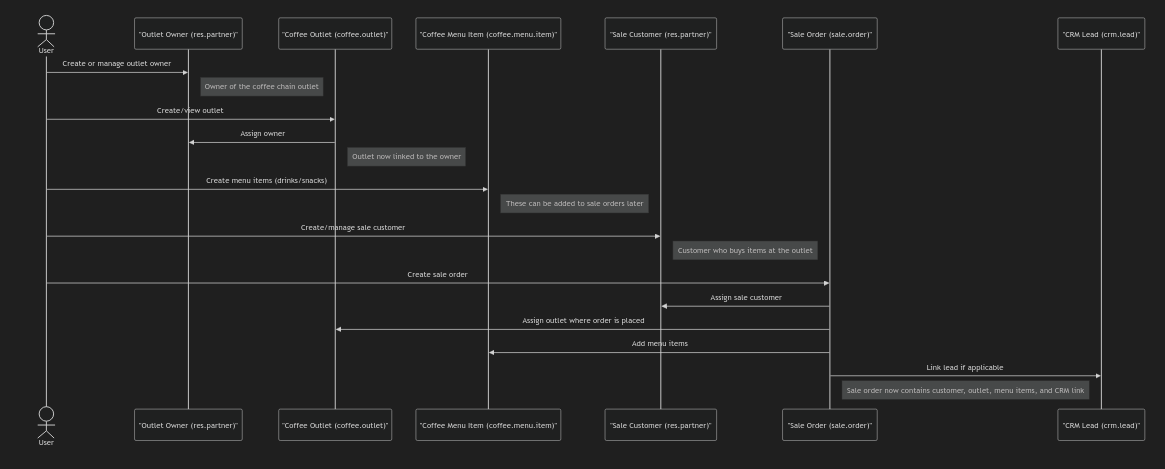
\includegraphics[width=1.0\textwidth,keepaspectratio]{diagrams/sequence.png}
\caption{Sequence Diagram: Sales Order Processing in Coffee Chain ERP}
\end{figure}
  % Chapter 7
\chapter{Code, Class, and Master Data Schema for Coffee Chain ERP System}

\section*{Introduction}
This chapter explains the master data structure and schema used in the Coffee Chain ERP system. It first introduces key terminologies for understanding ERP data models, then describes the master data entities, relationships, and schema as implemented in the system. This provides a foundation for understanding the system’s code and database structure.

\section*{Basic Terminologies}

\begin{description}
    \item[Entity:] A distinct object or concept in the system that stores data. Examples include Customer, Product, or Outlet.
    \item[Attribute:] A property or field of an entity. For example, a Customer entity may have attributes such as Name, Email, and Phone Number.
    \item[Primary Key:] A unique identifier for an entity instance. In Odoo, this is often the \texttt{id} field.
    \item[Relationship:] The association between two entities, such as One-to-Many or Many-to-One. Example: Each Outlet is owned by one Outlet Owner, while an owner can have multiple outlets.
    \item[Master Data:] Core data that is essential for the operation of a system, such as Customers, Products, and Outlets.
    \item[Business Logic Layer:] Code that defines the rules and behavior of the system, often implemented via Python classes in Odoo modules.
    \item[Model/Class:] In Odoo, a model is a Python class that defines the structure of an entity, including fields, relationships, and methods.
\end{description}

\section*{Master Data in Coffee Chain ERP System}
The Coffee Chain ERP system’s master data schema includes the following key entities:

\subsection*{Outlet Owner (\texttt{res.partner})}
\begin{tabular}{|l|l|l|}
\hline
\textbf{Field} & \textbf{Type} & \textbf{Description} \\
\hline
id & int & Primary Key \\
name & string & Owner Name \\
email & string & Contact Email \\
phone & string & Contact Number \\
\hline
\end{tabular}

\noindent
\textbf{Relationship:} One owner can manage multiple Coffee Outlets (One-to-Many).

\subsection*{Coffee Outlet (\texttt{coffee.outlet})}
\begin{tabular}{|l|l|l|l|}
\hline
\textbf{Field} & \textbf{Type} & \textbf{Description} & \textbf{Relationship} \\
\hline
id & int & Primary Key & — \\
name & string & Outlet Name & — \\
location & string & Outlet Address & — \\
owner\_id & int & Foreign Key & res.partner.id (Outlet Owner) \\
\hline
\end{tabular}

\noindent
\textbf{Relationships:} Many-to-One with Outlet Owner, One-to-Many with Sale Orders.

\subsection*{Coffee Menu Item (\texttt{coffee.menu.item})}
\begin{tabular}{|l|l|l|}
\hline
\textbf{Field} & \textbf{Type} & \textbf{Description} \\
\hline
id & int & Primary Key \\
name & string & Item Name \\
price & float & Item Price \\
category & selection & Drinks / Snacks \\
image & binary & Item Image \\
\hline
\end{tabular}

\noindent
\textbf{Relationship:} Many-to-Many with Sale Orders.

\subsection*{Sale Customer (\texttt{res.partner})}
\begin{tabular}{|l|l|l|}
\hline
\textbf{Field} & \textbf{Type} & \textbf{Description} \\
\hline
id & int & Primary Key \\
name & string & Customer Name \\
email & string & Contact Email \\
phone & string & Contact Number \\
\hline
\end{tabular}

\noindent
\textbf{Relationship:} One-to-Many with Sale Orders; optional link to CRM Leads.

\subsection*{Sale Order (\texttt{sale.order})}
\begin{tabular}{|l|l|l|l|}
\hline
\textbf{Field} & \textbf{Type} & \textbf{Description} & \textbf{Relationship} \\
\hline
id & int & Primary Key & — \\
order\_number & string & Unique Order Number & --- \\
customer\_id & int & Foreign Key & res.partner.id (Sale Customer) \\
outlet\_id & int & Foreign Key & coffee.outlet.id \\
order\_date & date & Order Timestamp & --- \\
\hline
\end{tabular}

\noindent
\textbf{Relationship:} Many-to-One with Sale Customer and Outlet; Many-to-Many with Menu Items; optional FK to CRM Lead.

\subsection*{CRM Lead (\texttt{crm.lead})}
\begin{tabular}{|l|l|l|l|}
\hline
\textbf{Field} & \textbf{Type} & \textbf{Description} & \textbf{Relationship} \\
\hline
id & int & Primary Key & — \\
lead\_name & string & Lead Title & --- \\
stage & string & Lead Status & — \\
related\_order\_id & int & Optional FK & sale.order.id \\
\hline
\end{tabular}

\noindent
\textbf{Relationship:} Optional linkage to Sale Orders and Sale Customers.

\section*{Master Data Schema Diagram}
The following diagram visually represents the **tables, fields, primary keys, and relationships** in the Coffee Chain ERP system:

%\begin{figure}[H]
 %   \centering
  %  \includegraphics[width=0.9\textwidth]{diagrams/masterdata_schema.png}
   % \caption{Master Data Schema showing entities, attributes, primary keys, and relationships.}
%\end{figure}

\section*{Python Classes Mapping to Master Data}
The ERP system implements the master data entities as Python classes in Odoo modules:

\begin{itemize}
    \item \texttt{coffee.outlet} → Python class \texttt{CoffeeOutlet(models.Model)}
    \item \texttt{coffee.menu.item} → Python class \texttt{CoffeeMenuItem(models.Model)}
    \item \texttt{res.partner} → Used for both Outlet Owner and Sale Customer
    \item \texttt{sale.order} → Python class \texttt{SaleOrder(models.Model)}
    \item \texttt{crm.lead} → Python class \texttt{CrmLead(models.Model)}
\end{itemize}

\subsection*{Field Definitions Example}
For example, the \texttt{CoffeeMenuItem} class defines the following fields:

\begin{lstlisting}[language=Python, caption={Coffee Menu Item Python Class}]
from odoo import models, fields

class CoffeeMenuItem(models.Model):
    _name = 'coffee.menu.item'
    _description = 'Coffee Menu Item'

    name = fields.Char(required=True)
    price = fields.Monetary(currency_field='currency_id', required=True)
    category = fields.Selection([
        ('drinks', 'Drinks'),
        ('snacks', 'Snacks'),
    ], required=True)
    image = fields.Image(max_width=128, max_height=128)
\end{lstlisting}

\begin{figure}[H]
    \centering
    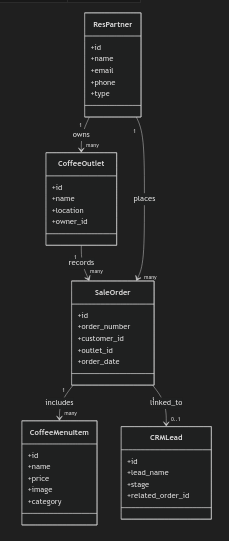
\includegraphics[width=0.356\textwidth]{diagrams/masterdata.png}
    \caption{Class diagram showing Python classes and field names for quick reference.}
\end{figure}

\section*{Summary}
The master data schema of the Coffee Chain ERP system ensures:

\begin{itemize}
    \item Clear separation of entities: outlets, menu items, customers, orders, and leads.
    \item Proper relationships to maintain data integrity: e.g., orders linked to customers and outlets.
    \item Python classes in Odoo accurately define the structure, fields, and relationships.
    \item The schema supports the business logic and workflow described in previous chapters.
\end{itemize}
             % Chapter 8
\chapter{Access Rights and User Roles in Coffee Chain ERP System}

\section*{Introduction}
Access control is a fundamental aspect of any ERP system. It ensures that users can only access data and perform actions according to their responsibilities. This chapter explains the concept of access rights, user roles, and how they are implemented in Odoo. Finally, it details the specific access rights configured for the Coffee Chain ERP system based on its code.

\section*{General Concepts: Access Rights and User Roles}
\begin{description}
    \item[Access Rights:] Define what operations a user can perform on data. These typically include:
        \begin{itemize}
            \item \textbf{Read:} View records.
            \item \textbf{Write:} Edit existing records.
            \item \textbf{Create:} Add new records.
            \item \textbf{Delete / Unlink:} Remove records.
        \end{itemize}
    \item[User Roles:] Groupings of users with similar responsibilities. A role determines which models and actions a user can access.
    \item[Role-Based Access Control (RBAC):] Common model where access is granted based on the user’s role rather than individual permissions.
\end{description}


\section*{Access Control in Odoo}
In Odoo, access rights are managed using:
\begin{itemize}
    \item \textbf{Groups:} Collections of users sharing the same role.
    \item \textbf{Models:} Entities like \texttt{res.partner}, \texttt{sale.order}, or \texttt{coffee.menu.item}.
    \item \textbf{Permissions:} Defined in \texttt{ir.model.access.csv}, specifying read, write, create, and delete rights for a group on a model.
\end{itemize}

Each record operation in Odoo checks:
\begin{enumerate}
    \item Whether the user belongs to a group with the necessary permission.
    \item Whether the record is accessible under record rules (not covered in this chapter but relevant for finer control).
\end{enumerate}

\section*{User Roles in Coffee Chain ERP System}
The Coffee Chain ERP system defines the following primary user roles:

\begin{itemize}
    \item \textbf{Outlet User:} Staff who manage outlet operations, including sales orders, POS transactions, accounting entries, and menu items.
    \item \textbf{CRM User:} Staff who manage CRM leads and related customer interactions.
    \item \textbf{Help User:} Users who only need read access to help documents and guides.
\end{itemize}

These roles are implemented in Odoo using groups such as \texttt{base.group.user} and custom groups defined in the modules.

\section*{Access Rights for Coffee Chain ERP System}
The following table presents a matrix of access rights for the models in the system, derived from the \texttt{ir.model.access.csv} files in the modules:

% Table 1: ID, Name, Model
\begin{table}[H]
\centering
\begin{tabular}{|p{6cm}|p{6cm}|p{5cm}|}
\hline
\textbf{ID} & \textbf{Name} & \textbf{Model} \\
\hline
access\_coffee\_outlet\_user & access.coffee.outlet.user & coffee.outlet \\
access\_crm\_lead\_inherit\_user & access.crm.lead.inherit.user & crm.lead \\
access\_res\_partner\_inherit\_user & access.res.partner.inherit.user & res.partner \\
access\_coffee\_help\_user & access.coffee.help.user & coffee.help \\
access\_coffee\_crm\_help\_user & access.coffee.crm.help.user & coffee.crm.help \\
access\_coffee\_sales\_help\_user & access.coffee.sales.help.user & coffee.sales.help \\
access\_sale\_order\_outlet\_user & access.sale.order.outlet.user & sale.order \\
access\_sale\_order\_line\_coffee\_user & access.sale.order.line.coffee.user & sale.order.line \\
access\_account\_move\_outlet\_user & access.account.move.outlet.user & account.move \\
access\_account\_payment\_outlet\_user & access.account.payment.outlet.user & account.payment \\
access\_pos\_config\_outlet & access.pos.config.outlet & pos.config \\
access\_pos\_order\_outlet\_user & access.pos.order.outlet.user & pos.order \\
access\_pos\_order\_line\_outlet\_user & access.pos.order.line.outlet.user & pos.order.line \\
access\_coffee\_menu\_item\_user & access.coffee.menu.item & coffee.menu.item \\
access\_coffee\_menu\_tag\_user & access.coffee.menu.tag & coffee.menu.tag \\
\hline
\end{tabular}

\end{table}

% Table 2: Model continuation
\begin{table}[H]
\centering
\begin{tabular}{|p{5cm}|p{4cm}|c|c|c|c|c|}
\hline
\textbf{Model} & \textbf{Group} & \textbf{Read} & \textbf{Write} & \textbf{Create} & \textbf{Delete} \\
\hline
coffee.outlet & base.group.user & 1 & 1 & 1 & 1 \\
crm.lead & base.group.user & 1 & 1 & 1 & 1 \\
res.partner & base.group.user & 1 & 1 & 1 & 1 \\
coffee.help & — & 1 & 0 & 0 & 0 \\
coffee.crm.help & — & 1 & 0 & 0 & 0 \\
coffee.sales.help & — & 1 & 0 & 0 & 0 \\
sale.order & — & 1 & 1 & 1 & 1 \\
sale.order.line & — & 1 & 1 & 1 & 1 \\
account.move & — & 1 & 1 & 1 & 1 \\
account.payment & — & 1 & 1 & 1 & 1 \\
pos.config & base.group.user & 1 & 1 & 0 & 0 \\
pos.order & base.group.user & 1 & 1 & 1 & 1 \\
pos.order.line & base.group.user & 1 & 1 & 1 & 1 \\
coffee.menu.item & — & 1 & 1 & 1 & 1 \\
coffee.menu.tag & — & 1 & 1 & 1 & 1 \\
\hline
\end{tabular}
\caption{User Access Rights Matrix for Coffee Chain ERP System}
\end{table}




\section*{Explanation of Key Permissions}
\begin{itemize}
    \item Outlet-related models (\texttt{coffee.outlet}, \texttt{sale.order}, \texttt{pos.order}, etc.) have full CRUD access for staff responsible for operations.
    \item CRM models (\texttt{crm.lead}) allow full management for CRM users.
    \item Help-related models (\texttt{coffee.help}, \texttt{coffee.crm.help}, \texttt{coffee.sales.help}) are read-only to prevent modification by general users.
    \item POS configuration (\texttt{pos.config}) is restricted from creation to avoid accidental setups.
    \item Coffee menu items and tags can be fully managed by outlet staff to ensure menu updates.
\end{itemize}

\section*{Practical Examples of Access Control}

To better illustrate how access rights operate in practice:

\begin{itemize}
    \item A \textbf{regional manager} can view performance reports for multiple outlets but cannot directly edit outlet menus or prices. This ensures visibility without risking accidental changes to operational data.
    \item An \textbf{employee} (e.g., barista) can create sales orders and process transactions in the POS system but cannot modify outlet profiles or assign outlet managers. This limits their permissions to day-to-day operational tasks only.
    \item A \textbf{CRM user} can manage leads and customer interactions but cannot delete accounting entries or modify sales orders, keeping financial data protected.
\end{itemize}

These examples show how the system enforces the principle of least privilege, ensuring that each role has exactly the access needed to perform its duties, no more and no less.


This chapter explains general concepts of access rights and user roles, how they are implemented in Odoo, and the specific permissions configured for the Coffee Chain ERP system. The matrix provides a clear reference for developers, system administrators, and auditors to understand role-based access control within the system.
          % Chapter 9

\end{document}
